%%%%%%%%%%%%%%%%%%%%%%%%%%%%%%%%%%%%%%%%%%%%%%%%%%%%%%%%%%%%%%%%%%%%%%%%%%%%%%%%%%
\documentclass[12pt]{article}
\usepackage{graphics}
\usepackage{graphicx}    	% needed for including graphics e.g. EPS, PS
\usepackage{subfigure}
\usepackage{amsmath}

\usepackage[colorlinks, bookmarks=false]{hyperref}
\hypersetup{
    colorlinks,
    citecolor=black,
    filecolor=black,
    linkcolor=black,
    urlcolor=black
}
\topmargin -1.5cm        	% read Lamport p.163
\oddsidemargin -0.04cm   	% read Lamport p.163
\evensidemargin -0.04cm  	% same as oddsidemargin but for left-hand pages
\textwidth 16.59cm
\textheight 21.94cm 
%\pagestyle{empty}       	% Uncomment if don't want page numbers
\parskip 7.2pt           	% sets spacing between paragraphs
%\renewcommand{\baselinestretch}{1.5} % Uncomment for 1.5 spacing between lines
\parindent 0pt		 				% sets leading space for paragraphs%%%%%%%%%%%%%%%%%%%%%%%%%%%%%%%%%%%%%%%%%%%%%%%%%%%%%%%%%%%%%%%%%%%%%%%%%%%%%%%%%%

\newcommand{\degree}{\ensuremath{^\circ}}

\title{Handr\'{e}: An Experimental Approach to Intelligent Character/Word Recognition using Support Vector Machines \& Dynamic Time Warping}
\date{\today}
\author{
	Sang Woo Jun \\ 
	wjun@mit.edu \\ 
  \and
  Chong-U Lim\\
  culim@mit.edu
}

\begin{document}

\maketitle

\begin{abstract}

	In this report, we describe Handr\'{e}, a full-system implementation of an experimental approach to intelligent character/word recognition using support vector machines and dynamic time warping. Handr\'{e} is unique in that it attempts to use various computer font data instead of actual handwriting to approximate handwriting recognition. Our system implements three large subsystems. (1) Image segmentation using a time series edge detection method, (2) character recognition using both support vector machines and K-means clustering using dynamic time warping, and (3) word recognition using spelling correction. Our system was tested on professor Leslie Kaelbling's handwritten lecture notes. Even though out system includes various novel and experimental ideas, and suboptimally implemented in many areas due to lack of time and experience, our results showed resonable accuracy and promise.
	
\end{abstract}

\newpage
\tableofcontents
\newpage
\section{Introduction}

	Optical Character Recognition (OCR) is the term used to describe the process of recognizing scanned images of text from documents, which may be handwritten manuscripts or printed text. An extension to OCR is Intelligent Character Recognition (ICR), which involves additional processing and recognition techniques in order to improve the accuracy of translating such documents by performing recognition on the level of words as opposed to individual characters. In this paper, we present an experimental system to outline the process of performing recognition of an entire handwritten document. Our approach outlines the feasibility of performing word recognition without having to collect hand-written samples for training. We make use of a windowed time-series edge detection method and pixel analysis to perform segmentation of the document invididual words and characters respectively. To perform individual character recognition, we used 2 different approaches -- a kernel-based support vector machine (SVM) classifier and a K-means clustering method using dynamic time-warping (DTW) which were both trained using a database of TrueType fonts. We then perform a committee based process of combining results from both models together with a probablistic spelling checker in order to perform the word recognition. 

\subsection{Emphasis}
	We emphasize the following multiple of Handr\'{e} unique characteristics.
	
	\paragraph{Feasibility of Font Training Data} We conduct exploratory work on using default computer fonts such as Verdana, Comic Sans MS, and handwriting-like fonts such as angelina and harrison to train our learning methods, instead of collecting a large corpus of handwritten characters for training. Results show that this is a feasible method
	
	\paragraph{Multiple Character Predictors} We use both SVM and DTW methods to predict characters, and merge them through a committee based process. Because SVM is more accurate with more training data and DTW is more accurate when there is less training data, our implementation works at a reasonable accuracy at various amounts of training data.
	
	\paragraph{Full-System Approach} Instead of implementing a subset of a complete working system, we attempted to implement the entire system stack, up to the point where it was actually usable. Because there were multiple cross-checking functionality such as the committee based merging and spelling correction, we could obtain a certain level of utility even when some of the individual functionality was incomplete.
	
	\paragraph{Feature-dtw} The K-means clustering method goes through multiple, each a tree in a forest of less-accurate classifiers. The first classifier is a novel variant of multi-dimendional dynamic time warping named feature-dtw, which generates two 'feature' time series by scanning the pixel layout according to the dimensions, and adding the distance between the two pairs. This method almost always assures that the correct character is included in the top ten or so of possible characters, speeding up all subsequent classifiers by multiple orders of magnitude by reducing the problem space.

\section{Segmentation}
\label{section:segmentation}
	\subsection{Word Segmentation}
		\subsubsection{Time-series Segmentation}
		A real-time edge detection method for times series was used to extract individual word images from a scanned image of a document. The image is first scanned vertically, constructing a time series consisting of the number of black pixels per vertical position. This information is analyzed to separate each lines into individual images. Each segmented line image is then scanned horizontally, constructing a time series. This is analyzed to segment individual words.
		
		In order to accurately segment lines and words, we adapted a time series edge detection method proposed to segment heartbeats to identify separating spaces between lines and words. This is done by first differentiating the time series and then doing a moving window integration, to discover the transition point separating the dense and sparsely colored regions. This generally resulted in more accurate results than simple pixel density analysis employed by most work.
		
		Figure~\ref{figure:word_segmentation} shows the plot of a processed time series derived from pixel density of a single line image and its resulting word segmentation. This image was taken from a screenshot of one of professor Leslie Kaelbling's lecture notes.
		
		\begin{figure}[htbp!]
		\centering
		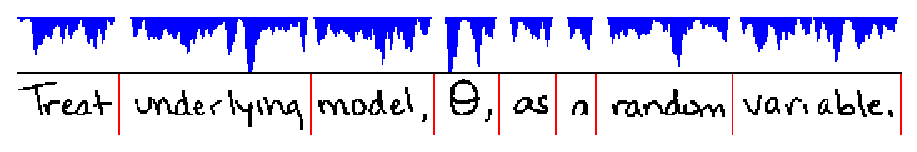
\includegraphics[width=0.7\textwidth]{word_segmentation.eps}
		\label{figure:word_segmentation}
		\caption{Word segmentation of an example line.}
		\end{figure}
		
		\subsubsection{Post-processing}
		Because scanned handwritten documents contain many types of noise information such as underlines and shadows, a certain amount of post-processing on the segmented word image to obtain relatively clean character data. First, single pixel noise was eliminated by removing pixel 'islands', that existed by itself with only one or no neighboring pixels. Second, underlines were removed by picking the top one or two horizontal lines with a very high pixel density and removing each pixel from it, unless it had pixels above and below it. Third, strokes spilled over from lines above one in interest was removed, by scanning all pixels on the first row of the image and recursively filling all adjacent black pixels with white.
		

	\subsection{Character Segmentation}
		Because individual characters in a handwritten word often have overlapping widths or just plainly connected, the same method of using pixel density cannot be used to segment characters in a word. Furthermore, it is provably impossible to perfectly segment characters in a word without symantic context. For example, it is just as likely for 'm' to be segmented into 'm', as it is to be segmented into 'rn' or any other subsection of 'm' that may not exist in the english alphabet.
		
		However, because this research is a preliminary feasibility search that does not heavily focus on character segmentation, we employed some preprocessing by hand and simple pixel analysis to perfectly segment characters in a word. First, word images were preprocessed by hand, by deleting some pixels so that no characters are touching each other. Then, simple pixel analysis was used to exploit this feature and correctly segment characters. This method was useful because it was much more productive than hand segmenting every character manually.

			
\section{Recognition}
\label{section:recognition}
	In this section, we outline the techniques which we focused on in order to address recoginition task of our project. In Section~\ref{subsection:svm}, we describe desribe support vector machines (SVM) and how they can be used for classification of the different alpha-numerical characer by training on a dataset in order to learn a model which generalizes well for all characters.. Section~\ref{subsection:dtw} covers dynamic time warping, and describes our approach to using it to classify alpha-numerical characters by minimising the distance of difference between the pixel-representations of the different characters. Section~\ref{subsection:spellingcheck} explains how a spelling checker is implemented in order to act as a type of regularization of the combined results from the SVM and DTW systems.

	\subsection{Classification using Support Vector Machines}	
	\label{subsection:svm}
	Support Vector Machines (SVMs) are a form of supervized learning methods which can be used for classificaiton or regression problems. In a binary classification example, we would train the SVM on a labelled dataset and if they they are linearly separable, the SVM will find a unique separation boundary in the form of a hyperplane with points falling on each side having different classifications. The separation boundary would be one in which the margin is maximised. 

	In general, not all data points will be linearly separable often as a result of overlapping class-conditional probabilities. Also, there is a chance of overfitting on the training data points which might negatively affect the generalizability of the classifier for future points. As such, we adopt the use of \textit{slack variables} which results in a `soft margin', in which we allow some data points to be incorrectly misclassified with a certain penalty with the aim of overcome overfitting. The general formulation of SVMs as constained quadratic programming problem is as follows

	\begin{equation*}
	\label{equation:svm}
	\begin{aligned}
	& \underset{\theta}{\text{minimize}}
	& & C\sum_{i=0}^n\xi_{i} + \frac{1}{2} \parallel\mathbf{\theta}\parallel^{2}  \\
	& \text{subject to}
	& & y_{i}(\theta\cdot\mathbf{x}_{n}+\theta_{0}) \ge 1 - \xi_{i}, \; i = 1, \ldots, m
	\end{aligned}
	\end{equation*}

	where $x_{i}$ represents each training data point, with $y_{i}$ being its corresponding target classification. $\mathbf{\theta}$ is the model, or parameter, of the classifier with offset $\theta_{0}$, while C and $\xi$ represent the penalty and slack variables respectively.
	
	\paragraph{Supporting Multiple Classes}
	In our project, we are interested in the use of SVMs to classify individual characters based the a given vector input of pixel values. Extending SVMs to support multiple target classifications requires us to train multiple binary classifiers, one for each individual target character. Given an input vector, each classifier would give a possible classification, and we then employ \textbf{voting} as a way of deciding the best classification result for our data. The common voting strategies to decide on a classification described as follows. 	In \textbf{one-versus-one} voting, the idea is to fit a classifier for each pair of classes, and when it comes to making the prediction, we select the class with the most number of votes. In \textbf{one-versus-rest} voting, each character has a classifier which is fit to it. When making the predicition, the class with the highest classification output is chosen in a \textit{winner-takes-all} strategy.

	\subsection{K-means Clustering using Dynamic Time-Warping}
	\label{subsection:dtw}
	The second method used for character recognition is K-means clustering, using modified dynamic time warping as a distance metric. K-means clustering is an efficient method to use when classifying an input to one of the K possible clusters, which is a good fit to character recognition. Dynamic time warping (DTW) is a dynamic programming method to calculate the similarity between two time series by warping each time series into various ways to discover the warp configuration that makes the two series most similar. The difference between this method and normal euclidian distance can be seen in Figure~\ref{figure:dtw} This is also a good fit for character recognition because characters are generally similarly shaped, but it is stretched or warped in various ways. A window of ranges of warping allowed can be specified to aid in accuracy and speed.
	
	\begin{figure}[htbp!]
		\centering
		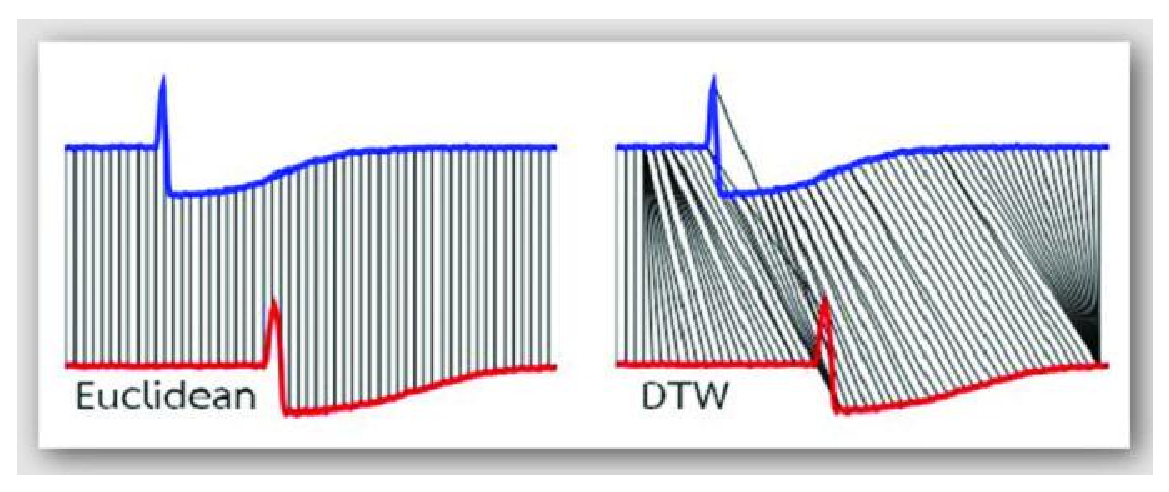
\includegraphics[scale=0.7]{dtw.eps}
		\label{figure:dtw}
		\caption{euclidian distance and dynamic time warping}
		\end{figure}
	
	\paragraph{Modified Dynamic Time Warping} We were unable to use multi-dimentional dynamic time warping for our goals, which is a common form of modified dynamic time warping used for image and texture analysis. Multi-dimentional dynamic time warping is done by taking the euclidian distance between each possible set of two rows, from both images and using dynamic time warping on it. However, this method could not be used because of two reasons. First, character sizes were often very different, making euclidian distance between rows not a very accurate measure. Second, it took a prohibitively long time.

	\begin{figure}[htbp!]
		\centering
		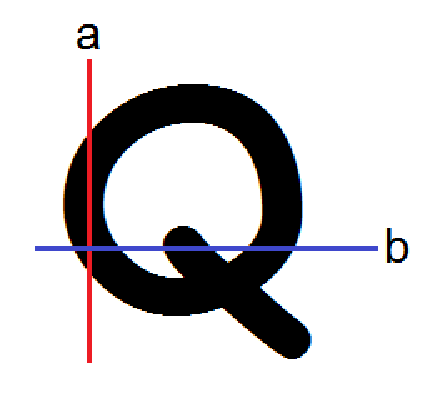
\includegraphics[scale=0.7]{xyfeatures.eps}
		\label{figure:xyfeatures}
		\caption{x and y features at position a and b}
		\end{figure}
		
	Therefore, we developed a novel method of character distance metric called feature-dtw, which has not been used in previous works, to the best of our knowledge. This method first generates two feature time series per character image, \textit{xfeature} and \textit{yfeature}, which are time series consisting of the number of pixel lumps that exists on that particular row or column. For example, in Figure~\ref{figure:xyfeatures}, the item in xfeature at index a would be 1, and the item in yfeature at index b would be 3. This feature series can be expected to have enough information in them, so when dynamic time warping is used on them, they can give a close approximation to the level of difference between two characters.
	
	Because feature-dtw is not completely accurate, it is only used as the first tree in a forest of classifiers, to first prune the problem space by taking the top 10 or so of most likely characters. Feature-dtw can often mistake some different characters to have the same features, depending on the tilt or shape of the characters. So after taking the top 10 or so of most likely characters from feature-dtw, traditional multi-dimentional dynamic time warping is used to actually classify the character.
	
	\paragraph {Modified K-means clustering} Because the level of difference between characters differ by lot, the default method of K-means clustering yielded multiple clusters with different characters in the same cluster, or with the same character split among different clusters. Therefore, we modified the K-means method to fit better into our ICR interface by picking character instances from different computer fonts that approximately separated the characters as much as possible, and using it as a 62-means cluster (26 + 26 upper- and lowercase letters and 10 digits).
	
	A problem arises from this configuration, because as shown above, certain character sets such as q and a are virtually indistinguishable from clustering, and will fall into the same cluster. (Experiments showed that the distribution of 'q' was larger than 'a', causing most 'a's to be classified as a 'q') The natural way to solve this would be to have a fewer number of clusters than characters at this point, and use Hidden Markov Models or some other method to guess the word. However, in order to maintain the same interface between DTW and SVM methods, the 62 means cluster was used without merging clusters, and it is sorted out during spelling correction. This results in several of the 62 clusters actually being interchangeable, and actually same clusters with multiple labels. Therefore, the predicted words may not look like actual words, but can be backtraced to predict the original correct word.

	\subsection{Combining Approaches for Word Recognition}
	\label{subsection:combined}
	We can improve the results of performing a classification task by including the results from a group of classifiers, as opposed to a single one. This is often termed as a \textit{committee}. We look to implement a form of committee-based decision by making use of the results from both the SVMs and feature-dtw methods when attempting to perform recognition on a character. In essence, each classificaton system will present a list of possible classification labels for a given input character, and by selectively pruning the sets into smaller subset, we hope to make a better informed decision on the classification. The exact process in which this is performed, along with the selection criteria and merging rules are both covered in Section~\ref{subsection:experiments:combinedchar}.


	\subsection{Spelling Correction Using Probalistic Dictionary Model}
	\label{subsection:spellingcheck}
	
	In order to account for the K-means clusters with different labels explained in section~\ref{subsection:dtw} and increase the accuracy of the final predicted words, we implement a modified version of the spelling corrector introduced in Peter Norvig's web site(***). This implementation of the spelling corrector works by reading a large number of words from a corpus and comparing them with input. Its speed is very fast because it works by generating a small number of possible corrections and matching them against an indexed database of corpus words. The spelling corrector in our system serves two functions.
	
	First, it corrects up to two mis-predicted characters in a predicted word. This is to increase the accuracy of predictions even with limited character recognition accuracy. If there are several possible matches, it first chooses the one with the least correct distance. If there is still a conflict, the one with the most occurrences in the corpus is chosen. Therefore, choosing a domain-specific corpus can improve accuracy. We used an entire body of words from a machine learning textbook as a corpus.
	
	Second, it understands that the 62-means clusters actually consists of much smaller number of clusters and only applied multiple labels and looks for interchangeable spellings that belong to the same cluster. Such multi-clusters include "e,c" "s,t,f" and "i,l". This creates a large number of possible permutation of corrections, but eventually finds the correct word.	
	
\section{Experimental Design}
\label{section:experiments}
In this section, we desribe the experimental design which we undertook in order to apply the segmentation and recognition techniques from Sections~\ref{section:segmentation} and~\ref{section:recognition}. In Section~\ref{subsection:experiments:svm}, we describe the prodedure in which we trained the multi-class SVMs on training data which consisted of different images of each alphabet character for a variety of fonts. Section~\ref{subsection:experiments:dtw} outlines the application of DTW onto a single font set and how it was used to perform its classification. How the results from both experiments were combined together to make committee-based decision is covered in Section~\ref{subsection:experiments:combinedchar}. Finally, Section~\ref{subsection:experiments:combinedword} explains the use of the dictionary spelling checker to improve the result and come up with a final decision.
	
	\subsection{Training \& Testing Data}
	For the purpose of our project, we tried to locate a resource of training data for alphabets which was commonly available. Several repositories containing data were either unsuitable or was paid-only. More importantly, we wanted to show-case that system could make use of a generic database for its training data, and not have to resort in having a particular target domain to have to first provide us with both a vast number of examples, but also go through the tedious task of hand-labelling them though it given the resources and time, it might be a possible way to improve the system (Section~\ref{section:conclusion}). As such, we decided to using readily available TrueType fonts as our training data.
			
		\subsubsection{Using Font Images as Training Sets}
		
		\begin{figure}[htbp!]
		\centering
		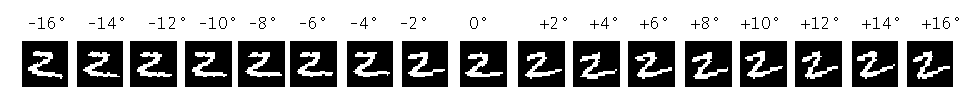
\includegraphics[width=0.8\textwidth]{training_data.eps}
		\caption{17 different rotations for each alphabet character}
		\label{figure:training_data}
		\end{figure}
		
		We made use of fonts for our training data by randomly picking a set of handwritten fonts which are freely available on the web (see Appendix~\ref{appendix:data:font} for the list and samples.) In order to normalize the characters, we resized each character to fit as a 28x28 white-on-black square image\footnote{We referenced the dimensions used by the MNIST database, and serves as a reference point for common handwritten character sizes.}. The character is then set to black-and-white mode, in which the pixel values are either 0 (black) or 255 (white). For each character in the font, we also created additional samples of the character image by rotating the characters by an angle between [-16\degree, +16\degree]. Thus, each training sample can be viewed as a 1x784 vector of pixel values. Figure~\ref{figure:training_data} shows an example of a font character which has been normalized and its various rotations.	
	
	\subsubsection{Testing on Handwritten Text}
		
		\begin{figure}[htbp!]
		\centering
		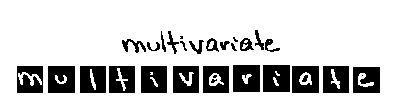
\includegraphics[width=0.5\textwidth]{multivariate_test.eps}
		\caption{Segmenting and normalizing a scanned image into its individual characters}
		\label{figure:multivariate_test}
		\end{figure}
		
		Image segments containing words which were obtained from the word-segmentation step (Section~\ref{section:segmentation}) were used for tests. The images were then cleaned and individual characters were extracted for the recognition process. We perform similar normalization steps in order to make the test images have the same dimensions and format as our training data -- images have their colors inverted, are cropped and resized to 28x28 pixels. Using our optimal performing classifier, we then attempt to classify each individual character in the word of $l$ characters. An example of a test image is shown in Figure~\ref{figure:multivariate_test}.
	
	\subsection{Recognizing Alphabet Characters using Multi-Class SVMs}
	\label{subsection:experiments:svm}

		In order to be train the best classifier for our recognition task, we varied the parameters and kernels used and performed cross-validation in order to select the best performing one. The following list describes the various parameters and choices we used

		\begin{itemize}
			\item Radial Basis Kernel
			\begin{itemize}
				\item C = [1, 10, 100, 1000]
				\item $\gamma$ = [0.01, 0.001, 0.0001]
			\end{itemize}
			\item Linear Kernel
			\begin{itemize}
				\item C = [0.001, 0.01, 0.01, 1, 10, 100, 1000]
			\end{itemize}
		\end{itemize}
		
		\begin{figure}[htbp!]
		\centering
		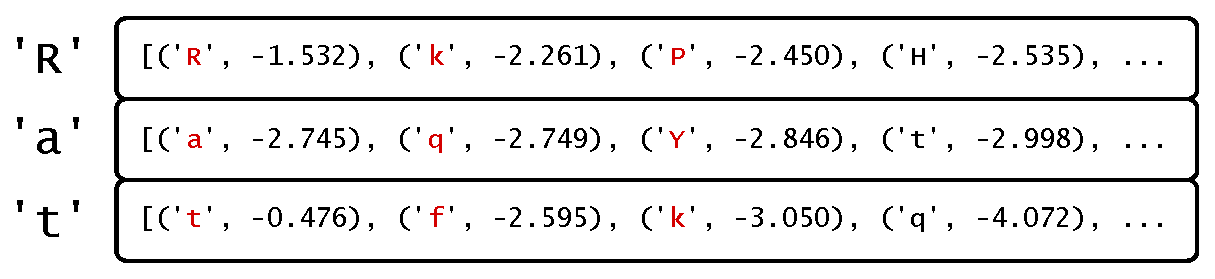
\includegraphics[width=0.8\textwidth]{svm_table.eps}
		\caption{An example of a prediction table after training on the scanned image containing the word `Rat'}
		\label{figure:svm_table}
		\end{figure}

		We optimised the parameters based on the precision score and recall score, and the results of which are shown in Section~\ref{subsubsection:analysis:svm}. Additionally, we made use of both the 1-versus-1 strategy and 1-versus-rest voting schemes to perform the multi-class classification. We also obtain the probability scores of each class (signifying how confident we are of our classification) to obtain a table containing $l$ rows, and each row contains a vector of 52 probabilities -- one each for the alphabets (26 upper-case and 26 lower-case characters.) As covered later in Section~\ref{subsection:experiments:combinedchar}, we will make use of this prediction table to make a combined decision, together with the DTW method, in order to improve our word recognition results. An example of a prediction table is shown in Figure~\ref{figure:svm_table}. In this case, the scanned image contains the word `Rat', and after classification of each character in the word, we assign a probabilistic score to each the possible classifications for the character. We use the log-probabilities due to some probabilities becoming extremely small. In the image, the rows are sorted from highest probable classification to lowest from left to right.

	
	\subsection{K-means Clustering using DTW}
	\label{subsection:experiments:dtw}
	
	After multiple experiments and cross validation, a 62 cluster means were chosen as a mixture of characters from fonts 'Verdana', 'Comic Sans MS' and a handwriting font 'angelina', all of which are freely available from the web. And among the several possible multi-clusters that have been discovered, the following five has been decided upon as a feasible compromise between accuracy and speed loss that results from the increasing number of possible permutations that arises from introducing more multi-clusters. This information is used by the spelling corrector to guess the possible original word.
	
	\begin{itemize}
		\item List of Chosen Multi-Clusters
		\begin {itemize}
			\item C1 = [a, q]
			\item C2 = [u, v, y]
			\item C3 = [c, e, f, t, r]
			\item C4 = [i, l]
			\item C5 = [h, n]
		\end {itemize}
	\end {itemize}
	
	For the dynamic time warping method, a window of 8 was used to specify the maximum amount of pixels each pixel can be warped, both for feature DTW and multi-dimensional DTW.
	

	\subsection{Combined Character Recognition}
	\label{subsection:experiments:combinedchar}
		
	With the resulting probability tables from the trained SVMs (Section~\ref{subsection:experiments:svm}) and the DTWs (Section~\ref{subsection:experiments:dtw}), we then developed a policy to select the resulting individual characters. First, each row in the probability was ordered from high to low -- with the most likely prediction in the front. Next, each character to be classified in the target string, we selected a subset from both the tables as a combined prediction by taking the intersection of the two sets. In the event that no characters are common between the two sets, we picked the most likely members from each set. 
	
	\begin{figure}[htbp!]
	\centering
	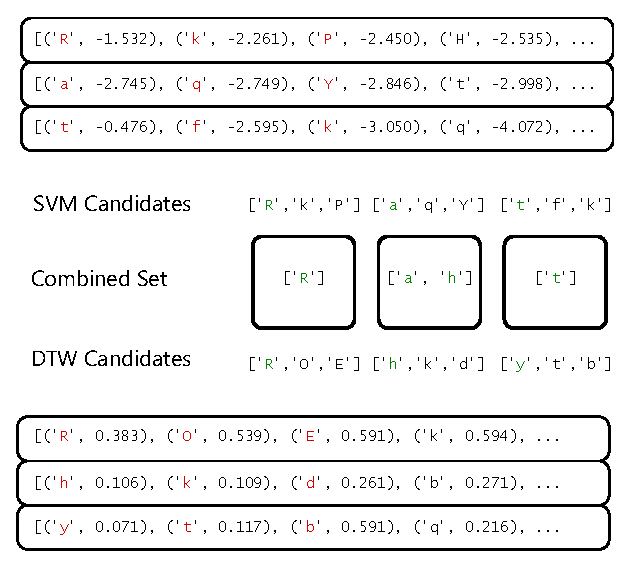
\includegraphics[width=0.6\textwidth]{combined_predictions.eps}
	\caption{Illustrating how predictions from both systems are combined.}
	\label{figure:combining_characters}
	\end{figure}
	
	
	This is illustrated in Figure~\ref{figure:combining_characters}. In this example, the scanned image contains the word `Rat'. The prediction table for the SVM system is shown at the top, while the table for the DTW system is at the bottom. For each character to be guessed, a subset of the top 3 predicted characters are chosen from both tables, so for the first character, we have the set $['R', 'k', 'p']$ and $['R', 'O', 'E']$ from the SVM system and DTW system respectively. Then, the intersection of the subets are assigned for first character of `Rat', which is `R'. For the second character, as there are no intersecting characters, we pick the top two predictions to form the subset $['a', 'h']$. The third character `t' follows the same discussion as the first character `R'.
	
	After some experimentation, we emperically decided that selecting subset of 3 characters from each prediction table row was the best policy due to potentially large number of permutations that might result from taking more. In the case where the intersecting set is empty, we picked the top predicted character from each of the tables.
	
\subsection{Word Recognition Using Spelling Correction}
	\label{subsection:experiments:combinedword}
	From the the result from the combined prediction, we may now have several permutations of guesses of the word which we wish to recognise. In this case, several constraints can be assumed to be true, notably that the length of the word has been correctly identified and that any mis-recognition which might have occured is entirely due to a substitution error in the given word string. As such, we make use of the spelling correction technique described in Section~\ref{subsection:spellingcheck} to the set of possible guesses for the word.  
	
	Following on our example from the previous section, we would have two potential guesses for the word -- `Rat' and `Rht'. In this case, if the spelling checker runs on the former, it would give a successful result and return, without a need to consider the second case. However, imagine the scenario that the resulting words were instead `Ret' and `Rat. In this case, the spelling checker would note that neither words exist, but attempt to propose a possible solution, which would be `Rat'. This provides an additional measure to contribute some form or prior knowledge into helping our classifiers make a classification, which both initially got wrong, eventually make a correct prediction.
	
	Because 'a' is part of the multi-cluster C1 and 'h' is part of the multi-cluster C5 introduced in section~\ref{subsection:experiments:dtw}, the spelling corrector would also check for possible spellings of 'Rqt' and 'Rnt'. However, because the corrector would already have returned with 'Rat' this path will not be taken in this example.	
	
\section{Results \& Analysis}
\label{section:results}
	In this section, we provide the results from the experiments conducted for the project which were explained in Section~\ref{section:experiments}. 
	
	\subsection{Alphabet Character Recognition using SVMs}
	\label{subsubsection:analysis:svm}
	
	\begin{figure}[htbp!]
	\centering
	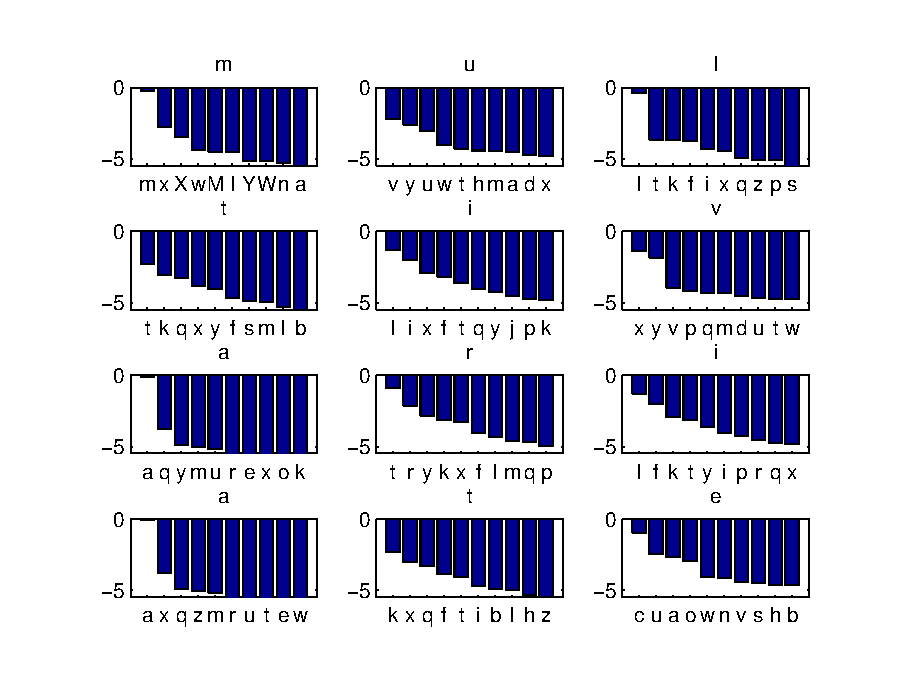
\includegraphics[width=0.8\textwidth]{svm_result.eps}
	\caption{Results of the SVM for the world `multivariate'. Larger values are better guesses.}
	\label{figure:svm_result}
	\end{figure}
	
	Lorem ipsum dolor sit amet, consectetur adipiscing elit. Quisque posuere molestie metus. Suspendisse tellus urna, porta sit amet rutrum eu, tristique quis urna. Donec varius pharetra purus, eget mollis tortor ornare vel. Nullam sagittis tellus id dui placerat eget congue libero facilisis. Donec mattis sagittis lectus, eget porta quam facilisis vel. Vestibulum non urna ante, nec mattis mauris. Nulla sit amet interdum eros. Nam congue lacinia nulla, vitae aliquet nisl tincidunt vel. Morbi gravida bibendum ipsum, at accumsan nisl suscipit ac. Sed accumsan cursus tortor a faucibus. Phasellus tempus, orci ac lacinia hendrerit, dui justo accumsan mi, congue dapibus massa turpis at lectus. Cras a tellus nisi. Aliquam vitae dolor id nunc lacinia fermentum et sit amet metus. Nullam viverra ante eu mauris ultrices nec adipiscing lectus dapibus. Class aptent taciti sociosqu ad litora torquent per conubia nostra, per inceptos himenaeos. Nam mollis commodo lacus, eget bibendum risus lobortis nec.
	
	\subsection{K-means Clustering using DTW}
	
	\begin{figure}[htbp!]
	\centering
	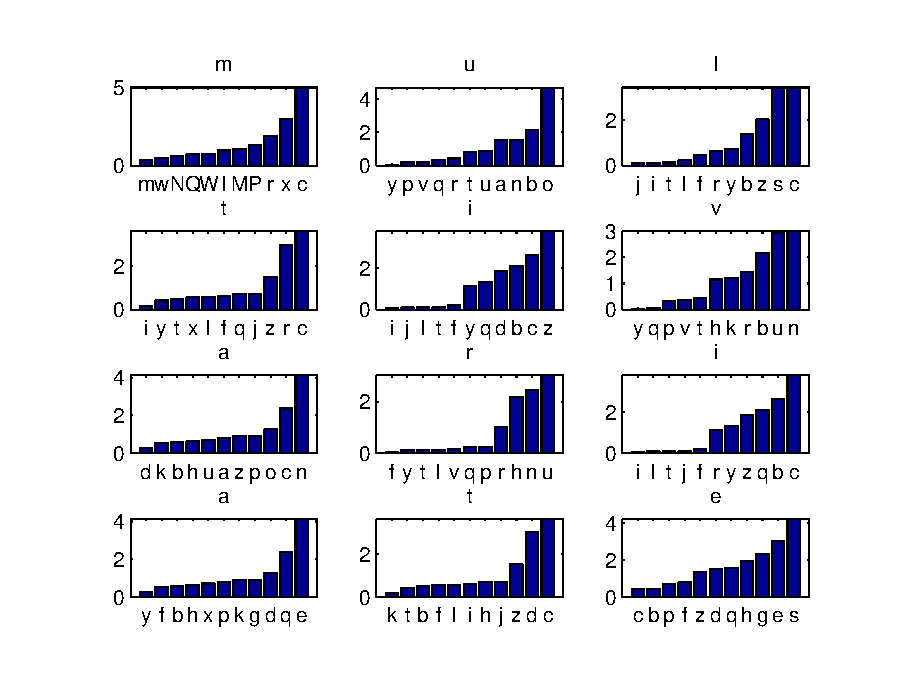
\includegraphics[width=0.8\textwidth]{dtw_result.eps}
	\caption{Results of the feature-DTW for the world `multivariate'. Smaller values are better guesses.}
	\label{figure:dtw_result}
	\end{figure}
	
	Lorem ipsum dolor sit amet, consectetur adipiscing elit. Quisque posuere molestie metus. Suspendisse tellus urna, porta sit amet rutrum eu, tristique quis urna. Donec varius pharetra purus, eget mollis tortor ornare vel. Nullam sagittis tellus id dui placerat eget congue libero facilisis. Donec mattis sagittis lectus, eget porta quam facilisis vel. Vestibulum non urna ante, nec mattis mauris. Nulla sit amet interdum eros. Nam congue lacinia nulla, vitae aliquet nisl tincidunt vel. Morbi gravida bibendum ipsum, at accumsan nisl suscipit ac. Sed accumsan cursus tortor a faucibus. Phasellus tempus, orci ac lacinia hendrerit, dui justo accumsan mi, congue dapibus massa turpis at lectus. Cras a tellus nisi. Aliquam vitae dolor id nunc lacinia fermentum et sit amet metus. Nullam viverra ante eu mauris ultrices nec adipiscing lectus dapibus. Class aptent taciti sociosqu ad litora torquent per conubia nostra, per inceptos himenaeos. Nam mollis commodo lacus, eget bibendum risus lobortis nec.
	
	\subsection{Combined Character Recognition}
	Lorem ipsum dolor sit amet, consectetur adipiscing elit. Quisque posuere molestie metus. Suspendisse tellus urna, porta sit amet rutrum eu, tristique quis urna. Donec varius pharetra purus, eget mollis tortor ornare vel. Nullam sagittis tellus id dui placerat eget congue libero facilisis. Donec mattis sagittis lectus, eget porta quam facilisis vel. Vestibulum non urna ante, nec mattis mauris. Nulla sit amet interdum eros. Nam congue lacinia nulla, vitae aliquet nisl tincidunt vel. Morbi gravida bibendum ipsum, at accumsan nisl suscipit ac. Sed accumsan cursus tortor a faucibus. Phasellus tempus, orci ac lacinia hendrerit, dui justo accumsan mi, congue dapibus massa turpis at lectus. Cras a tellus nisi. Aliquam vitae dolor id nunc lacinia fermentum et sit amet metus. Nullam viverra ante eu mauris ultrices nec adipiscing lectus dapibus. Class aptent taciti sociosqu ad litora torquent per conubia nostra, per inceptos himenaeos. Nam mollis commodo lacus, eget bibendum risus lobortis nec.
	
	\subsection{Word Correction}
	Lorem ipsum dolor sit amet, consectetur adipiscing elit. Quisque posuere molestie metus. Suspendisse tellus urna, porta sit amet rutrum eu, tristique quis urna. Donec varius pharetra purus, eget mollis tortor ornare vel. Nullam sagittis tellus id dui placerat eget congue libero facilisis. Donec mattis sagittis lectus, eget porta quam facilisis vel. Vestibulum non urna ante, nec mattis mauris. Nulla sit amet interdum eros. Nam congue lacinia nulla, vitae aliquet nisl tincidunt vel. Morbi gravida bibendum ipsum, at accumsan nisl suscipit ac. Sed accumsan cursus tortor a faucibus. Phasellus tempus, orci ac lacinia hendrerit, dui justo accumsan mi, congue dapibus massa turpis at lectus. Cras a tellus nisi. Aliquam vitae dolor id nunc lacinia fermentum et sit amet metus. Nullam viverra ante eu mauris ultrices nec adipiscing lectus dapibus. Class aptent taciti sociosqu ad litora torquent per conubia nostra, per inceptos himenaeos. Nam mollis commodo lacus, eget bibendum risus lobortis nec.
	
	\subsection{Example Results}
	
	\begin{figure}[htbp!]
	\centering
	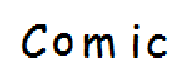
\includegraphics[width=0.5\textwidth]{comic_comp.eps}
	\caption{Computer-generated testing data}
	\label{figure:comic_comp}
	\end{figure}
	completely accurate
	
	\begin{figure}[htbp!]
	\centering
	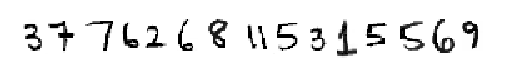
\includegraphics[width=0.5\textwidth]{number.eps}
	\caption{Testing data of digits}
	\label{figure:number}
	\end{figure}
	first 7 and second 3 was each recognized as 1 and 5.
	Important because spelling correction cannot be applied to digits
	
	
	\begin{figure}[htbp!]
	\centering
	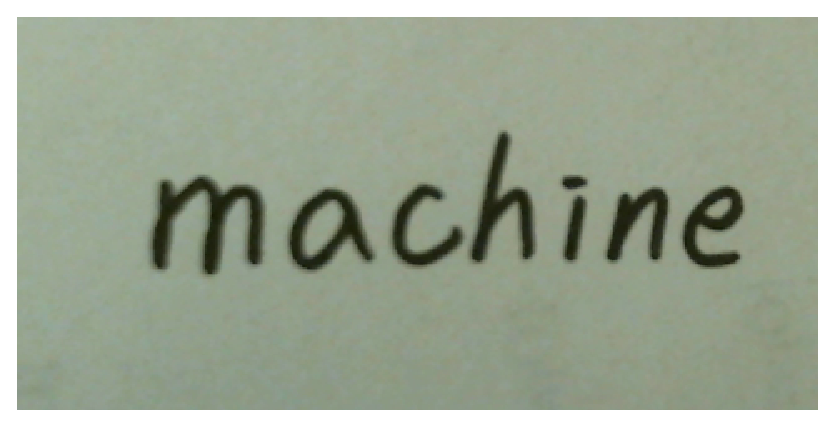
\includegraphics[width=0.5\textwidth]{machine_camb.eps}
	\caption{Handwritten text captured using webcam}
	\label{figure:machine_camb}
	\end{figure}
	
	\begin{figure}[htbp!]
	\centering
	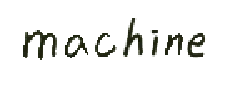
\includegraphics[width=0.5\textwidth]{machine_cam.eps}
	\caption{Preprocessed handwritten text}
	\label{figure:machine_cam}
	\end{figure}
	got 'mqchinc' on top
	
\section{Conclusions \& Future Work}
\label{section:conclusion}
	\subsection{Contributions}
	Contributed repository of training fonts as well as app to do it.
	Exhibited Feasibility of using Fonts as training data for SVMs.
	Showed positive results for combining different predictors.
	Novel feature-DTW approach for recognition.
	\subsection{Conclusions}
	Lorem ipsum dolor sit amet, consectetur adipiscing elit. Quisque posuere molestie metus. Suspendisse tellus urna, porta sit amet rutrum eu, tristique quis urna. Donec varius pharetra purus, eget mollis tortor ornare vel. Nullam sagittis tellus id dui placerat eget congue libero facilisis. Donec mattis sagittis lectus, eget porta quam facilisis vel. Vestibulum non urna ante, nec mattis mauris. Nulla sit amet interdum eros. Nam congue lacinia nulla, vitae aliquet nisl tincidunt vel. Morbi gravida bibendum ipsum, at accumsan nisl suscipit ac. Sed accumsan cursus tortor a faucibus. Phasellus tempus, orci ac lacinia hendrerit, dui justo accumsan mi, congue dapibus massa turpis at lectus. Cras a tellus nisi. Aliquam vitae dolor id nunc lacinia fermentum et sit amet metus. Nullam viverra ante eu mauris ultrices nec adipiscing lectus dapibus. Class aptent taciti sociosqu ad litora torquent per conubia nostra, per inceptos himenaeos. Nam mollis commodo lacus, eget bibendum risus lobortis nec.
	\subsection{Future Work}
	Lorem ipsum dolor sit amet, consectetur adipiscing elit. Quisque posuere molestie metus. Suspendisse tellus urna, porta sit amet rutrum eu, tristique quis urna. Donec varius pharetra purus, eget mollis tortor ornare vel. Nullam sagittis tellus id dui placerat eget congue libero facilisis. Donec mattis sagittis lectus, eget porta quam facilisis vel. Vestibulum non urna ante, nec mattis mauris. Nulla sit amet interdum eros. Nam congue lacinia nulla, vitae aliquet nisl tincidunt vel. Morbi gravida bibendum ipsum, at accumsan nisl suscipit ac. Sed accumsan cursus tortor a faucibus. Phasellus tempus, orci ac lacinia hendrerit, dui justo accumsan mi, congue dapibus massa turpis at lectus. Cras a tellus nisi. Aliquam vitae dolor id nunc lacinia fermentum et sit amet metus. Nullam viverra ante eu mauris ultrices nec adipiscing lectus dapibus. Class aptent taciti sociosqu ad litora torquent per conubia nostra, per inceptos himenaeos. Nam mollis commodo lacus, eget bibendum risus lobortis nec.

\section{Acknowledgements}
	We would like to thank Dahua Lin for reviewing our initial project proposal, and subsequently taking time out of his busy schedule to meet with us and provide guidance and ideas on approaches to the project. Also, we thank Prof. Leslie Kaelbling for imparting her wisdom and stimulating our ethusiasm in the topics of machine learning. 
	 
\appendix
	\section{Data \& Results}
		\subsection{Font Samples}
		\label{appendix:data:font}
	\section{Project Timeline}
		\subsection*{Week 1: 10/28 -- 11/5 }
			\begin{itemize}
				\item{Submit project proposal}
				\item{Narrow down choices to one for the project}
				\item{Read up on related papers/books}
			\end{itemize}
		\subsection*{Week 2: 11/6 -- 11/12  }
			\begin{itemize}
				\item{Continue reading related works}
				\item{Word Segmentation investigation}
				\item{Numerical digit classification investigation}
			\end{itemize}
		\subsection*{Week 3: 11/13 -- 11/19}
			\begin{itemize}
				\item{Character segmentation}
				\item{Dynamic time-warping experiments}
				\item{Alphabet characters classification investigation}
			\end{itemize}
		\subsection*{Week 4: 11/20 -- 11/26}
			\begin{itemize}
				\item{Font database}
				\item{Dynamic time-warping for classification}
				\item{SVMs for training on fonts and classification}
			\end{itemize}
		\subsection*{Week 5: 11/27 -- 12/5}
			\begin{itemize}
				\item{Improving individual results}
				\item{Heuristics for combining both predictors}
				\item{Dictionary spell-correction}
				\item{Report writing}
			\end{itemize}

	\section{Division of Labor}
	
\bibliography{air-presentation}	
\bibliographystyle{unsrt}

\end{document}

%%%%%%%%%%%%%%%%%%%%%%%%%%%%%%%%%%%%%%%%%%%%%%%%%%%%%%%%%%%%%%%%%%%%%%%%%%%%%%%%%%
